\apendice{Documentación de usuario}

\section{Introducción}
En este apéndice vamos a ver como instalar y realizar todas las acciones necesarias para poder ejecutar el proyecto finalmente.

\section{Requisitos de usuarios}
El objetivo de esta sección es indicar aquellos requisitos necesarios para que el usuario pueda utilizar el proyecto.

\subsection{Reguisitos software}
Es necesario tener instalado el gestor de máquinas virtuales Oracle VM Virtual Box. Este gestor puede ser utilizado prácticamente en cualquier sistema operativo, soportando la mayoría de sistemas Windows, Linux, Mac OS X y Solaris. Dado que la máquina es de 64 bits, en ocasiones nos encontramos con que Virtual Box no nos permite crearla, por ello es necesario tener activadas las opciones de virtualización desde la BIOS.

\subsection{Requisitos hardware}
En lo concerniente al hardware necesitamos un sistema que pueda correr sin problemas la máquina virtual. Como requisito mínimo es necesario un sistema cuya memoria RAM disponible para la máquina sea de 512 MB de RAM. En cuanto al espacio libre de disco es necesario al menos 20 GB. El procesador debe ser un x86, cualquier Intel o AMD reciente debe valer\cite{requeriments_VirtualBox}.


\section{Instalación}
Se va a proporcionar un disco que contiene la máquina en el formato \textit{Open Virtualization Format} <<OVF>>, que es un servicio virtualizado de la máquina virtual. En Oracle VM VirtualBox en la parte superior pulsamos \textit{Archivo} e \textit{Importar servicio virtualizado} como vemos en la figura \ref{fig:SerVir}, se abrirá una ventana donde debemos seleccionar la ubicación del servicio virtualizado. Automáticamente se pasará a una ventana cn las preferencias de la máquina por defecto como podemos ver en la figura \ref{fig:NueMaqVir}, y pulsamos \textit{Importar}. Por defecto tenemos 1 GB de RAM, que resulta suficiente para que funcione la máquina, si aumentamos la RAM veremos como aumenta la fluidez del servicio virtualizado.

\begin{figure}
\centering
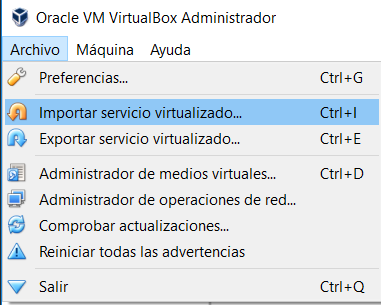
\includegraphics[width=.9\textwidth]{img/instalacion_user_servicio}
\caption{Importación de servicio virtual.}
\label{fig:SerVir}
\end{figure}

\begin{figure}
\centering
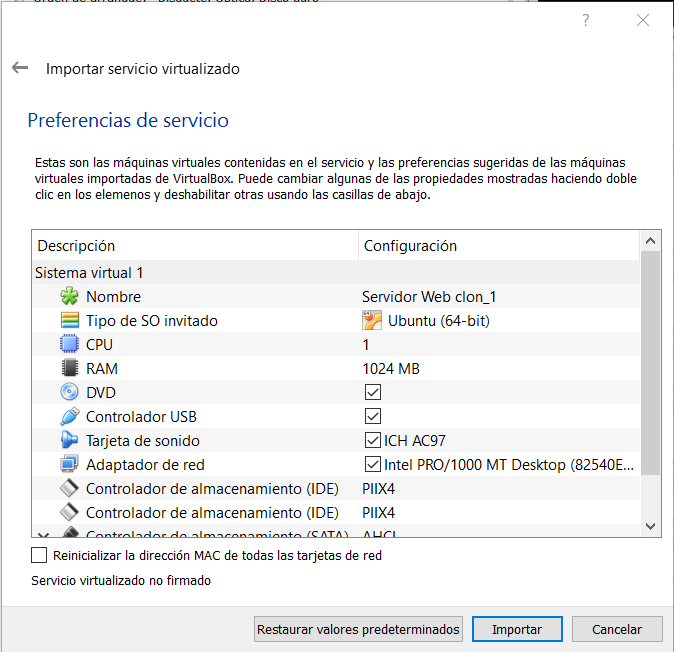
\includegraphics[width=.9\textwidth]{img/instalacion_user}
\caption{Preferencias del servicio virtual.}
\label{fig:NueMaqVir}
\end{figure}

Una vez iniciado es tan sencillo como abrir el Mozilla Firefox, cuyo icono encontramos a la izquierda en la barra de navegación de Ubuntu. Automáticamente debería abrirse en la página de inicio de nuestro sitio web, encaso de que no lo haga tecleamos en la barra de búsqueda \url{http://localhsot/inicio}. Una vez ya dentro, podremos utilizar el sitio web destinado.

\section{Manual del usuario}
El uso por parte del usuario de la aplicación web es muy sencilla, ya que las ejecuciones de los algoritmos están programadas por lo que no requiere intervención del usuario. El usuario se limita a observar los datos proporcionados por la interfaz, la interfaz es de sencillo uso y a continuación vamos a ver como utilizarla.

En la parte superior nos encontramos con una menú donde son 4 las opciones, como podemos observar en esta imagen\ref{fig:MenuDru}, y que vamos a describir brevemente:
\begin{figure}
\centering

\includegraphics[width=.9\textwidth]{img/drupal_menu}
\caption{Menú con el que puede interactuar el usuario.}
\label{fig:MenuDru}
\end{figure}

\begin{itemize}
\item \textbf{Inicio: } En esta opción nos encontramos con una breve descripción del proyecto y de las herramientas utilizadas.
\item \textbf{Informe General: } En este caso podemos observar del beneficio o pérdida obtenido en cada jornada y el balance global.
\item \textbf{Informe Jornada: } Si accedemos a través del menú podemos observar lo obtenido en una única jornada.
\item \textbf{Informe Pronóstico: } Nos proporciona los resultados que se esperan y las cuotas de las casas de apuestas.
\end{itemize}

Como podemos observar en la imagen, en esta primera página nos encontramos con la descripción del proyecto\ref{fig:IniDruUser}.

\begin{figure}
\centering
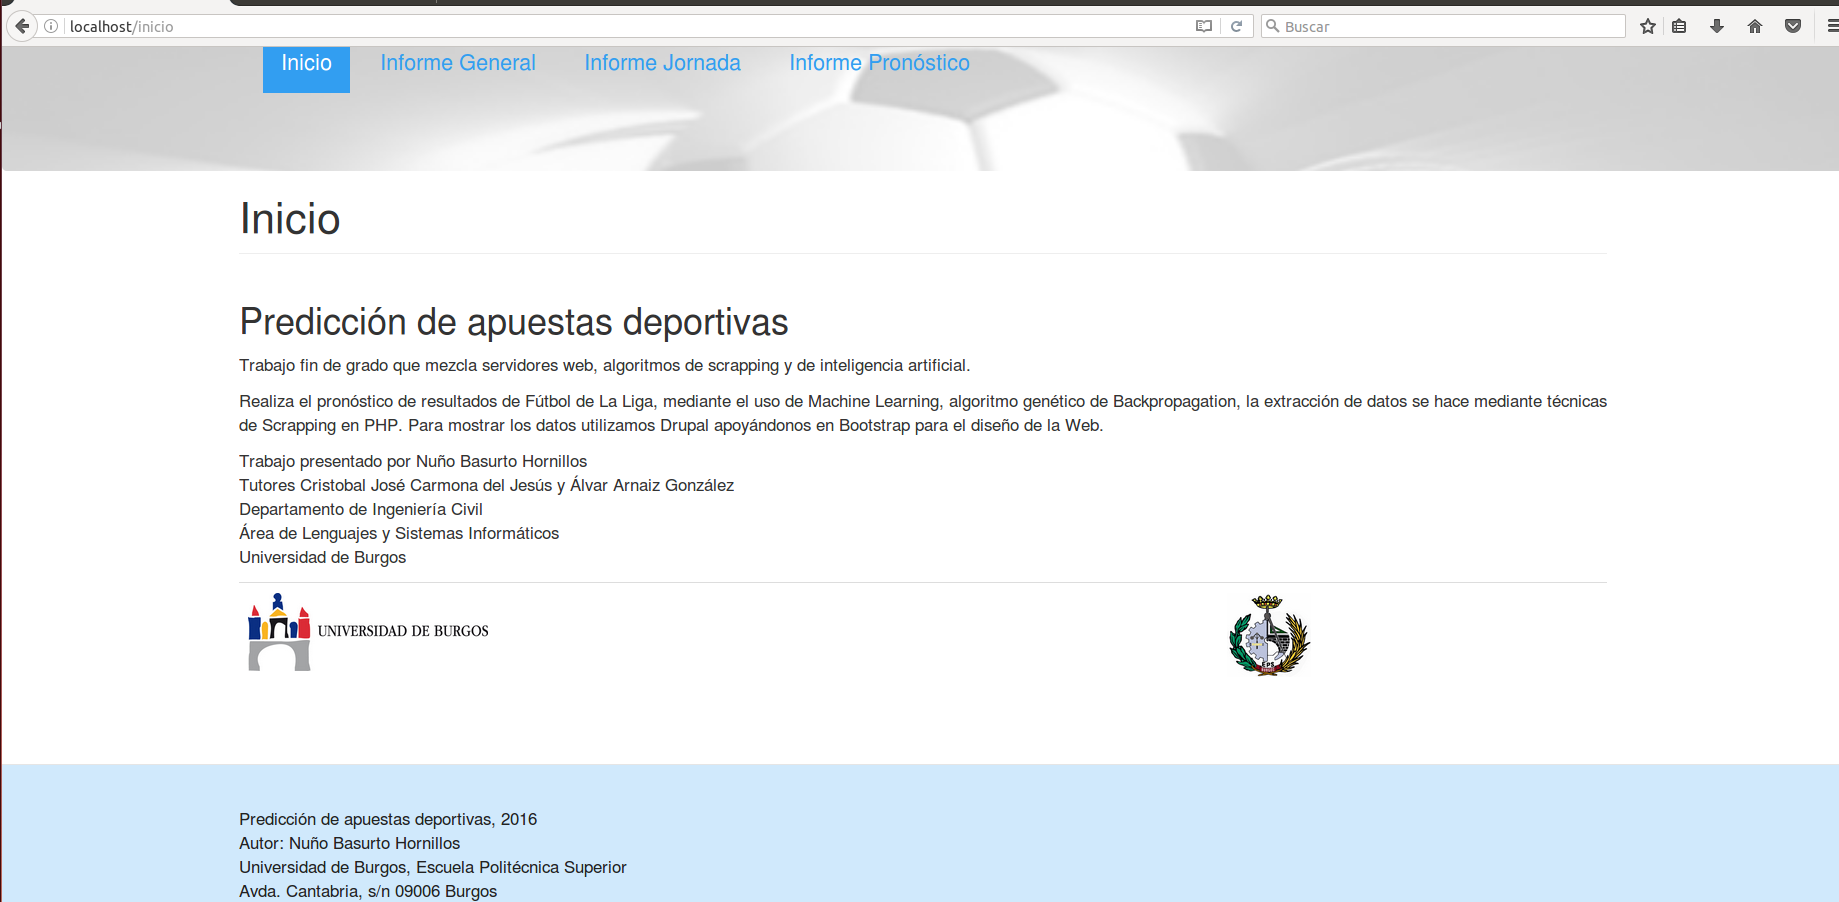
\includegraphics[width=.9\textwidth]{img/drupal_inicio_usuario}
\caption{Vista del usuario de Inicio.}
\label{fig:IniDruUser}
\end{figure}

En la ventana de informe general \ref{fig:InfGenDruUser}, podemos observar  una tabla con el balance de cada una de las jornadas, en cada una de las casas de apuestas, pulsando en la jornada accedemos a los partidos de la jornada más detalladamente, lo cuadros en verde son aquellos en los que se ha obtenido un balance positivo, en cambio encontramos en amarillo donde se pierde el dinero. Recordar que este es un balance por euro apostado. Por ejemplo en la jornada 14 observamos en la casa BET365 1.45 , entonces si apostásemos 10 en total (1 por partido) acabaríamos el día con 11.45, el 1.45 es el beneficio. En cambio en la jornada 15 en la misma casa de apuestas observamos -2.60, en este caso acabaríamos la jornada con 8.4, perdiendo dicho dinero.

\begin{figure}
\centering
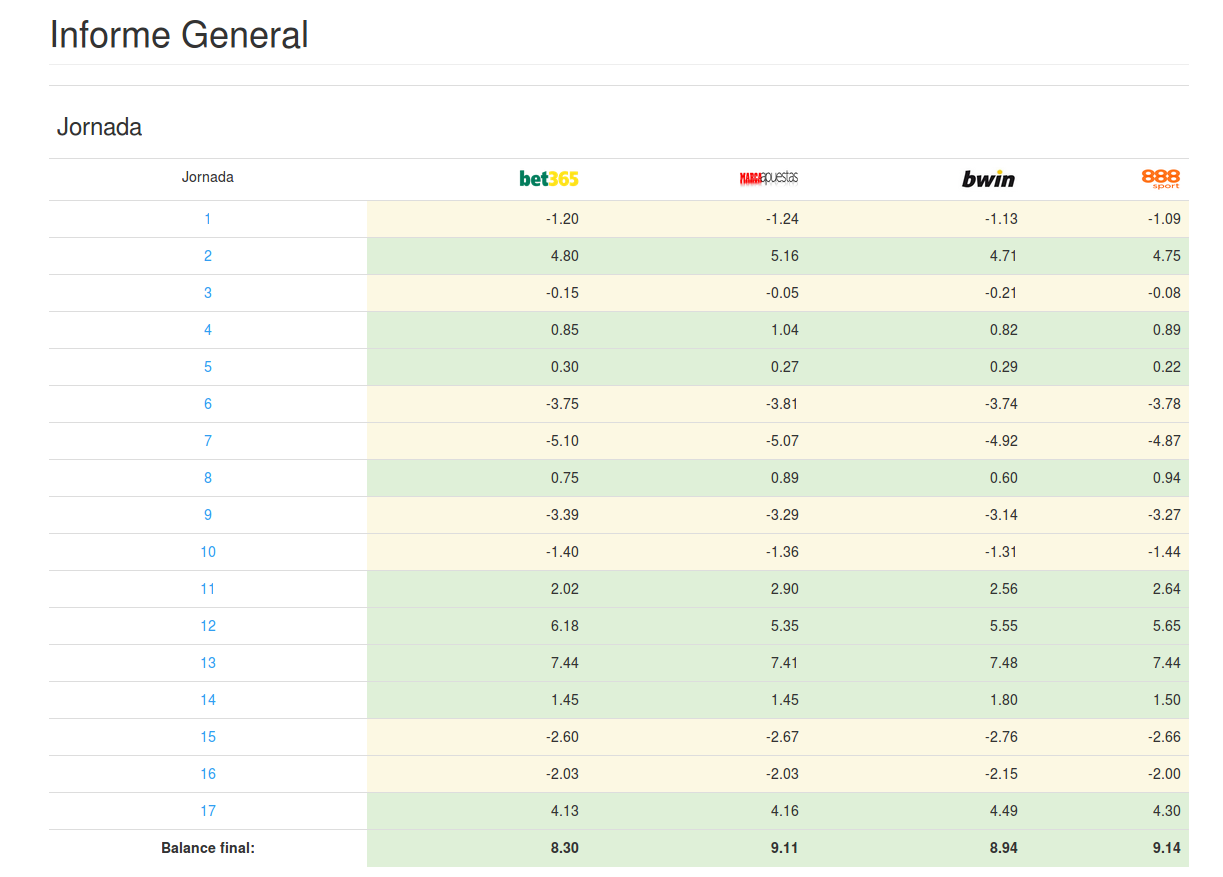
\includegraphics[width=.9\textwidth]{img/drupal_inf_general_usuario}
\caption{Vista del usuario del Informe de la Jornada.}
\label{fig:InfGenDruUser}
\end{figure}

A la ventana de Informe Jornada tenemos dos maneras de acceder, a través del menú donde observaremos el informe de la última jornada, o bien a través de los hipervínculos que encontramos en el Informe General, donde podemos acceder al resto de jornadas.
Podemos ves en negrita aquellos pronósticos que se han acertado, a su ves las casas de apuestas nos muestran lo predecido, mientras que aquellos partidos errados aparecen con -1 ya que el euro apostado en el partido se ha perdido. En la parte de abajo podemos observar el balance que veremos en amarillo si es negativo y en verde si es positivo.

En la imagen \ref{fig:InfJorDruUser}, observamos como la url es limpia por lo que nos muestra la última jornada a la que se ha accedido por el menú superior, en cambio si se ha accedido por el informe general veremos la imagen \ref{fig:InfJorDruUser2} con la URL diferente.

\begin{figure}
\centering
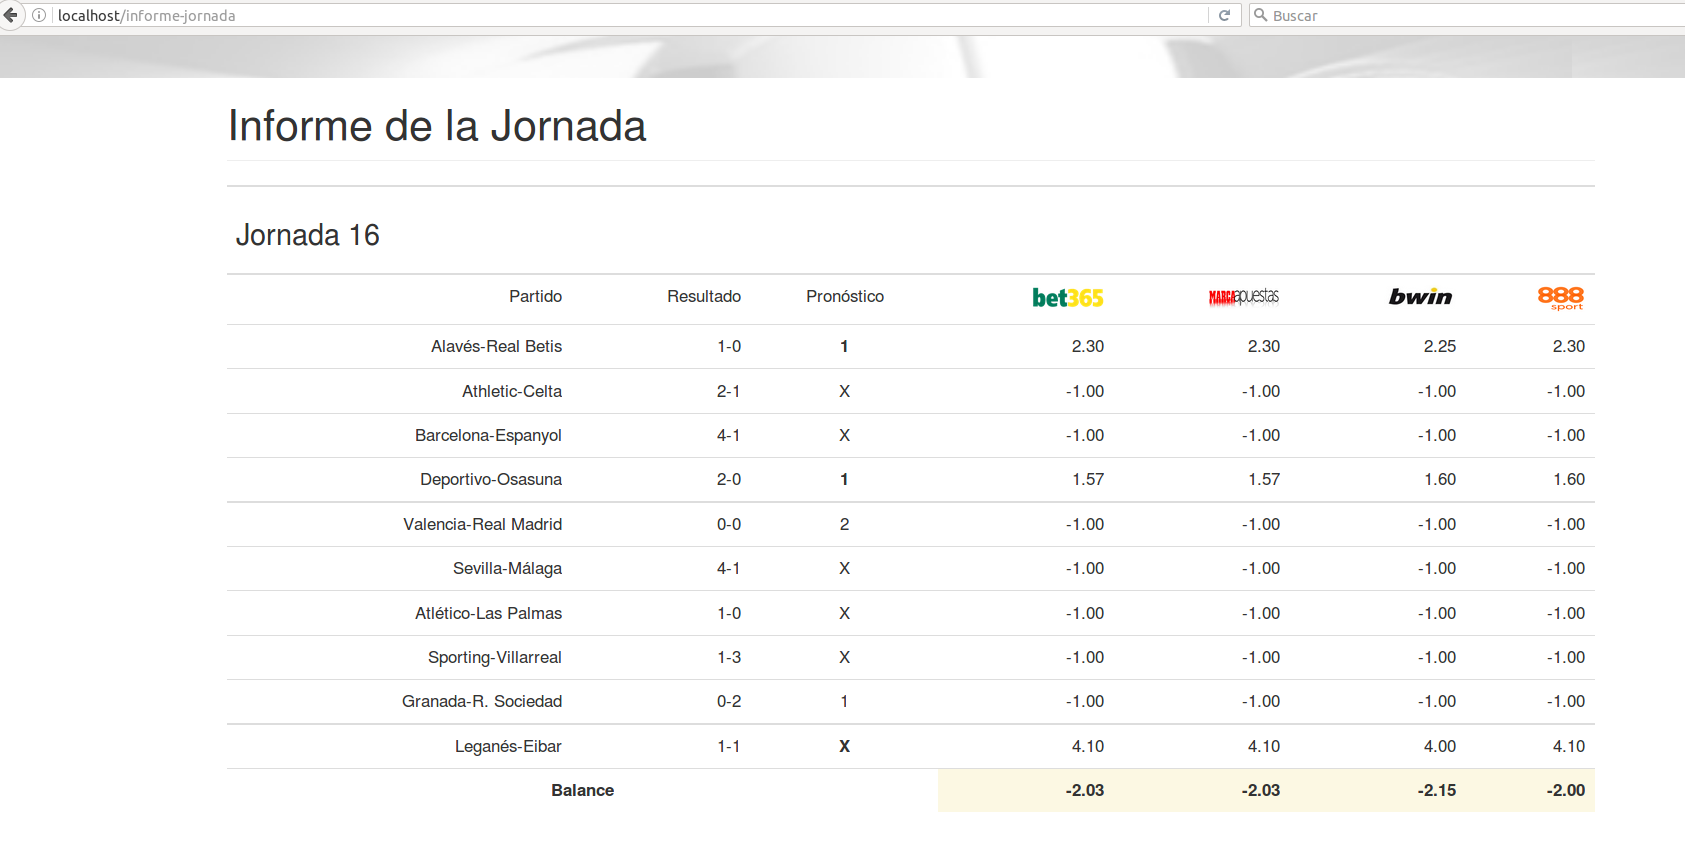
\includegraphics[width=.9\textwidth]{img/drupal_inf_jornada_usuario}
\caption{Vista del usuario del Informe Jornada.}
\label{fig:InfJorDruUser}
\end{figure}
\begin{figure}
\centering
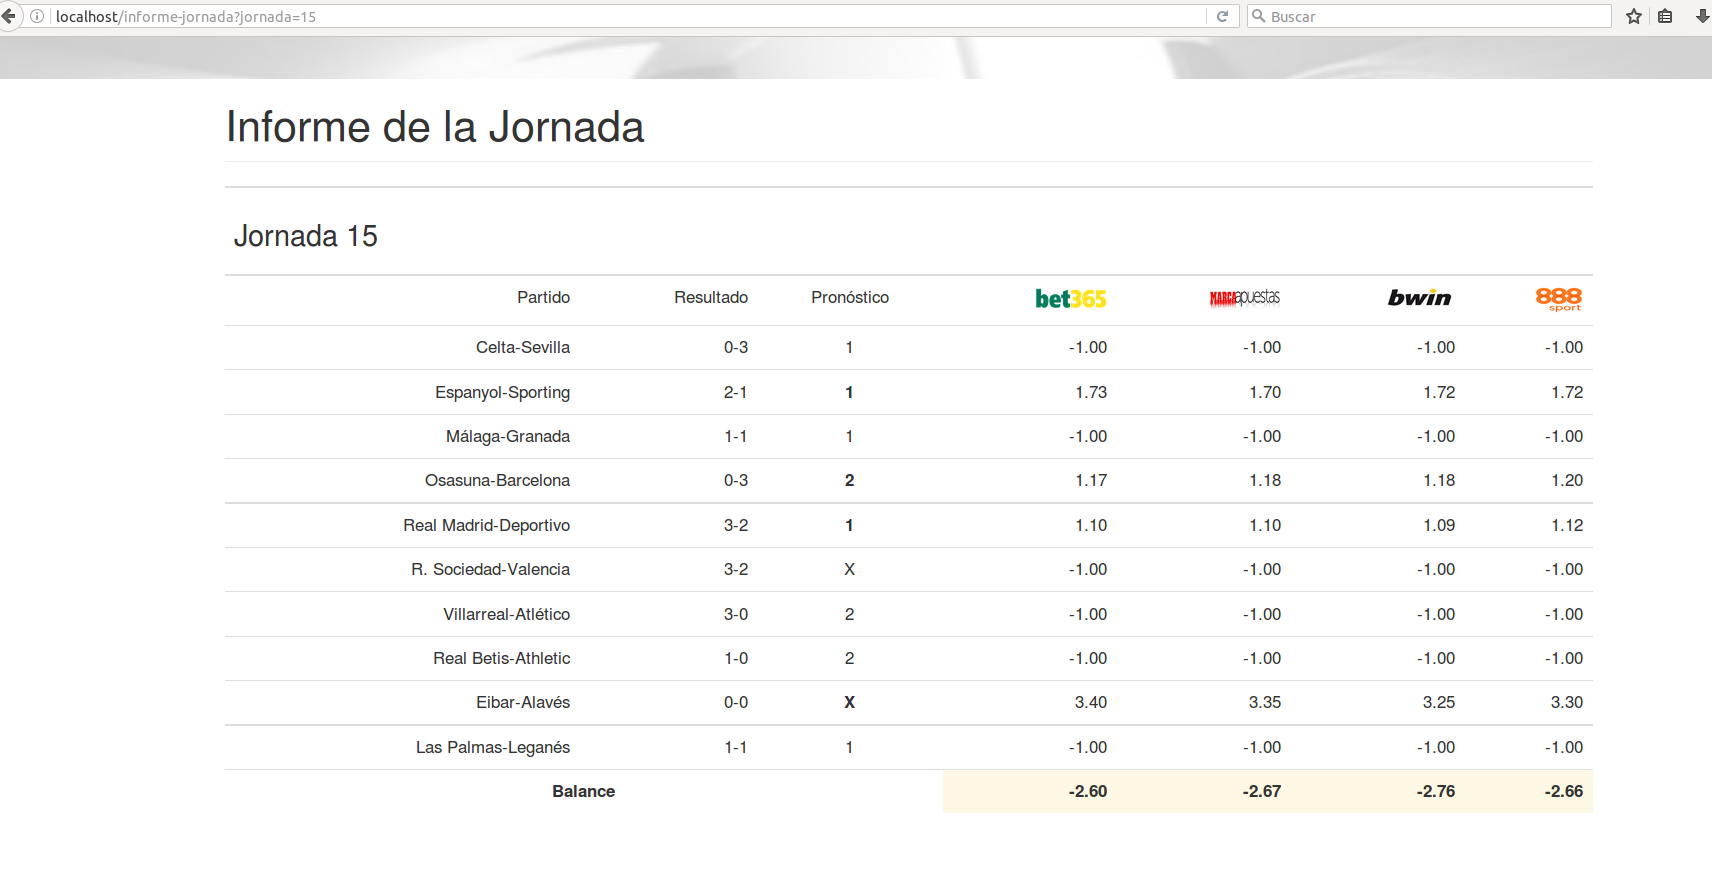
\includegraphics[width=.9\textwidth]{img/drupal_inf_jornada_usuario2}
\caption{Vista del usuario del Informe de la Jornada con la URL diferente.}
\label{fig:InfJor2DruUser}
\end{figure}

En el informe del pronóstico\ref{fig:InfProDruUser}, podemos observar todas las cuotas de los partidos para el pronóstico realizado. Y las ganancias potenciales que tenemos una vez finalizada la jornada se realizará el recuento y esta jornada pasará al informe de la jornada, poniendo aquí los partidos de la nueva jornada a la espera del pronóstico y de las cuotas de las casas de apuestas.

\begin{figure}
\centering
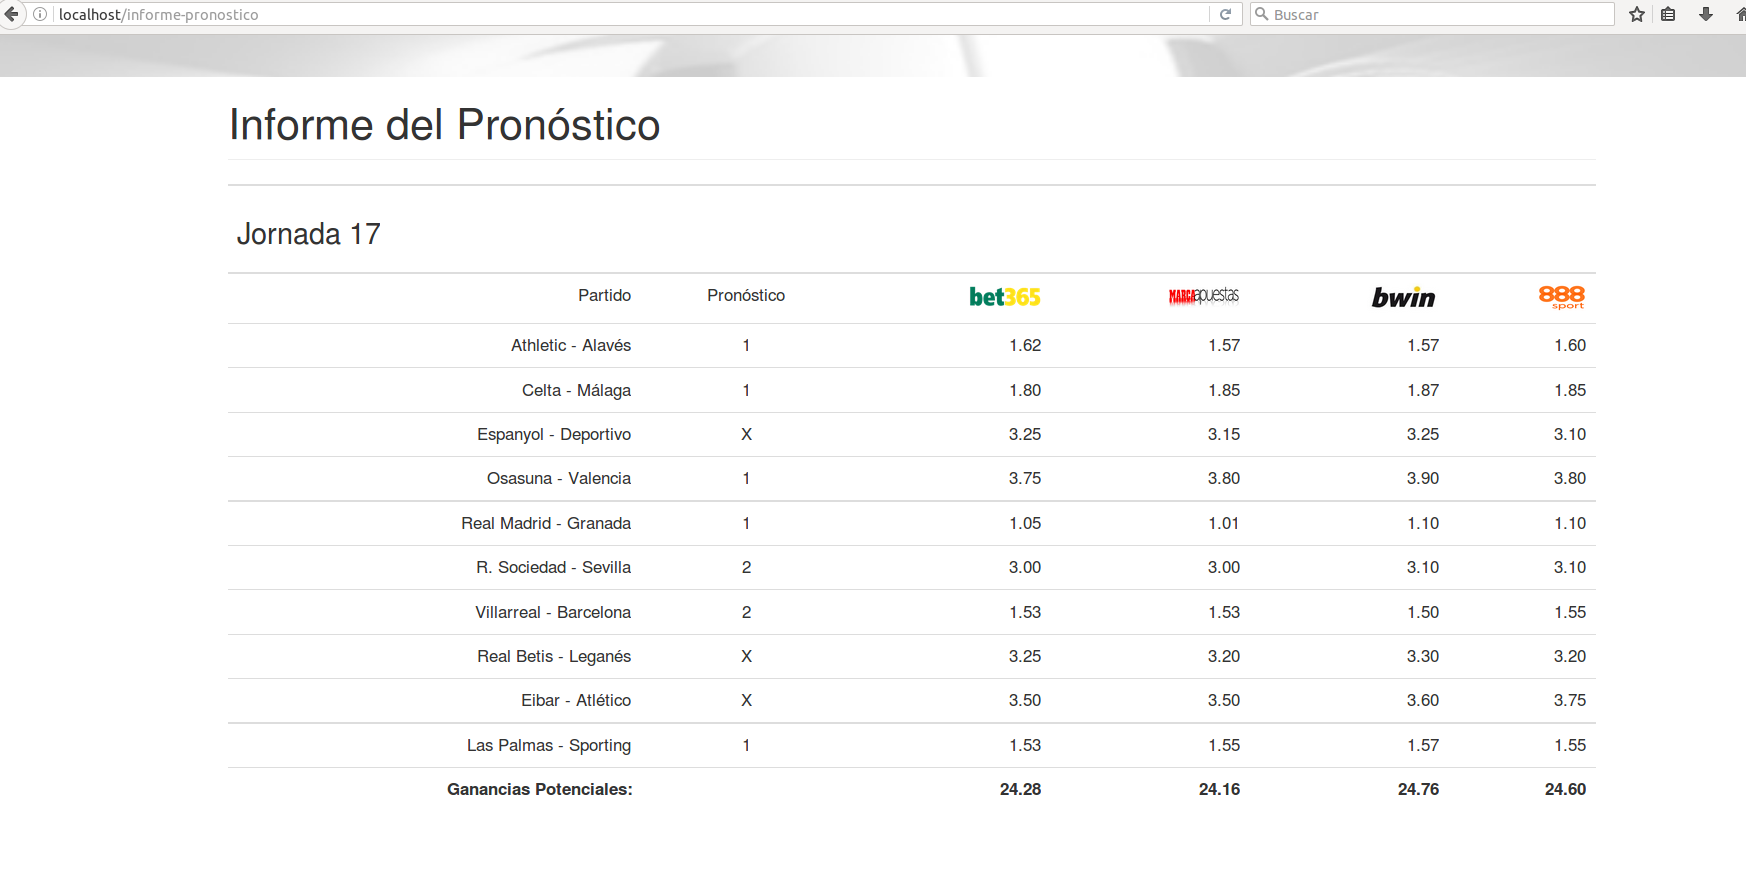
\includegraphics[width=.9\textwidth]{img/drupal_inf_pronostico_usuario}
\caption{Vista del usuario del Informe del pronóstico.}
\label{fig:InfProDruUser}
\end{figure}